% !Mode:: "TeX:UTF-8"
%%% Local Variables:
%%% mode: latex
%%% TeX-master: t
%%% End:

\chapter{基于生成对抗网络的遥感影像分割方法}
\label{cha:chap04}

\section{引言}
深度学习方法通过组合低阶特征形成更加抽象的高阶表示,基于全卷积架构的语义分割方法其多层的卷积网络结构可以完成对输入图像特征的自动学习。全卷积网络分割模型使用反卷积的上采样策略将特征图恢复到原始图像尺寸,完成对输入图像的像素级分类。然而,上采样过程造成了特征的损失,导致预测结果边界模糊的问题。另外,遥感影像由于其固有的信息不确定性,分类预测中地物边界模糊、歧义性等问题更加严重,全卷积语义分割方法在遥感影像分类中无法取得更佳的分类精度。
%同时,现有模型通常对每个像素类别进行预测,像素级别的准确率可能会很高,但是像素与像素之间的相关关系容易忽略,使得分割结果不够连续或者某个物体在分割结果中尺寸、形状与ground truth 图中的形状、尺寸差别较大。

生成对抗网络(Generative Adversarial Networks,GAN)训练时生成器(Genenrator)与判别器(Discriminator)不断对抗博弈,网络迭代好时判别器无法判断来源为生成器生成结果还是Ground truth 图,此时生成网络具有强大的图像生成能力\cite{luc2016semantic} 。本章将对抗网络应用到全卷积图像分割中,使得分割结果能够产生更好的地物边界,同类别物体空间上具有一致性。
%GAN 生成器生成原图的分割结果,GAN 判别器判断分割结果图来自Ground truth图还是生成器生成的语义分割结果。当判别器无法区分分割结果图的来源,ji


\section{基于生成对抗网络框架的影像分割方法}
\label{sec:firtst}

\subsection{生成对抗网络框架}
\label{sec:first-1}
GAN 是一种生成式的对抗网络,即通过对抗的方式,去学习数据分布的生成式模型。生成网络尽可能生成逼真样本,判别网络尽可能去辨别该样本是真实样本还是生成的假样本。

\begin{figure}[htb]
  \centering
  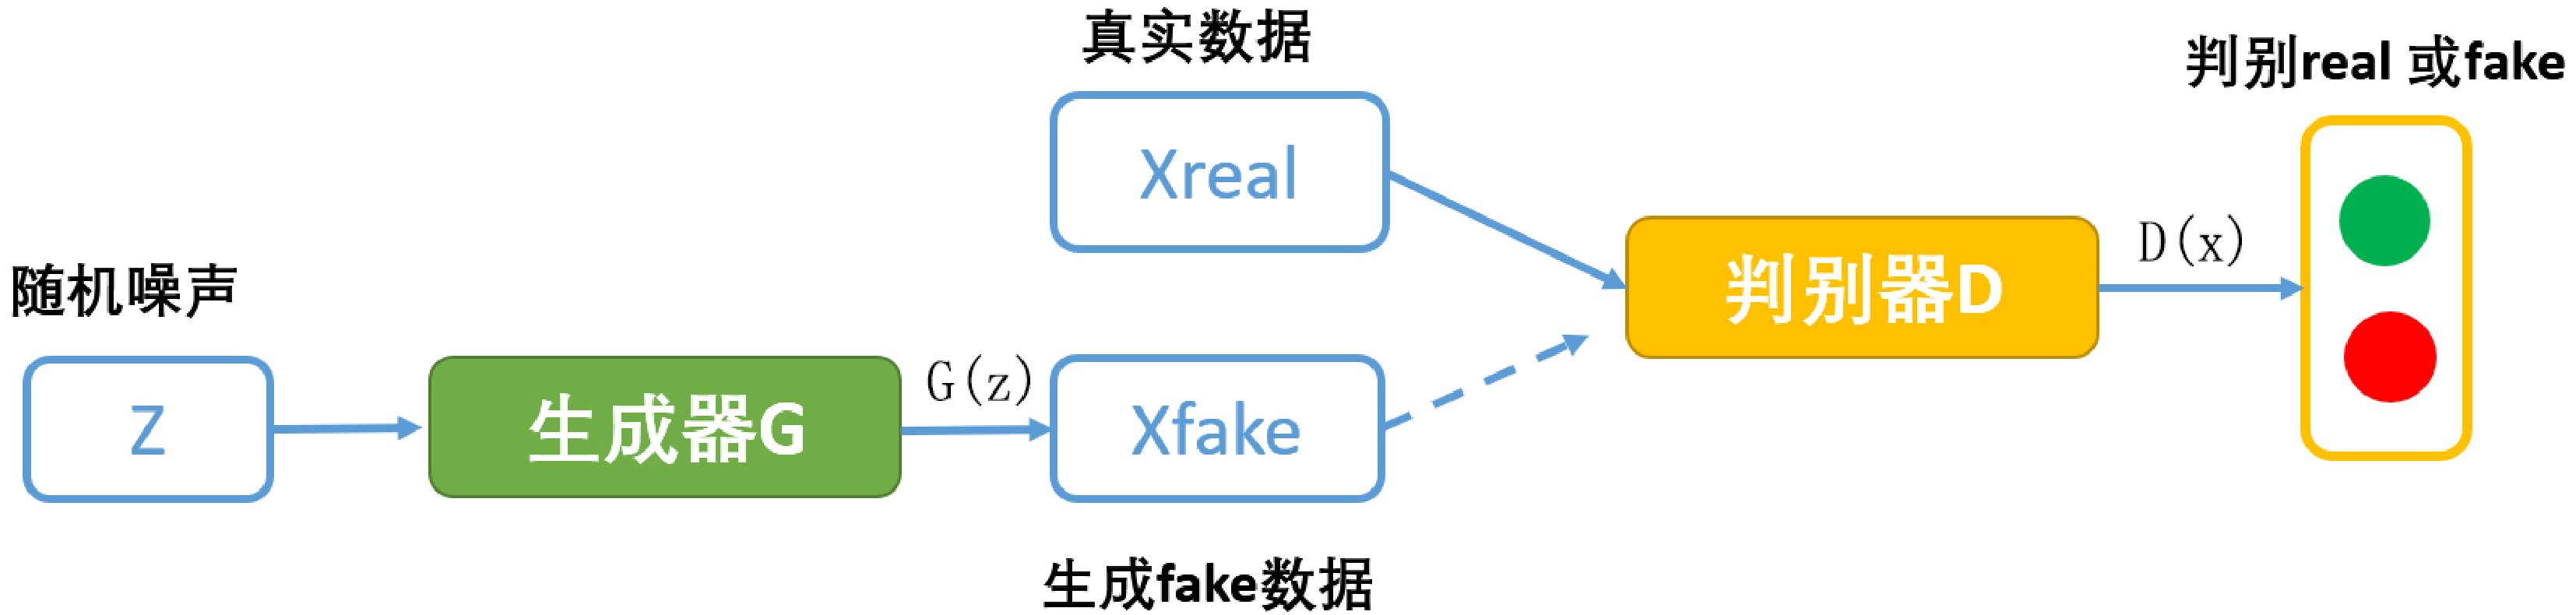
\includegraphics[width=0.8\textwidth]{figures/gan}
  \caption{GAN结构示意图}\label{fig:gan}
\end{figure}

如图\ref{fig:gan} 所示,假定变量$z$(通常为服从高斯分布的随机噪声)通过生成器G 生成$X_{fake}$,判别器D 负责判别输入的data 是生成的样本$X_{fake}$ 还是真实样本$X_{real}$。GAN 优化的目标函数为\ref{eq:4-1}:
\begin{equation}
  \label{eq:4-1}
  \mathop{\min}_{G} \mathop{\max}_{D} V(D,G) = \mathop{\min}_{G} \mathop{\max}_{D} E_{x \sim p_{data}(x)} [\log D(x)] + E_{z \sim p_{z}(z)}[ \log (1-D(G(z)))]
\end{equation}

式中$x \sim p_{data}(x)$ 表示$x$ 取自真实的分布数据。对于判别器D 来说,这是一个二分类问题,$ V(D,G)$ 为二分类中常见的交叉熵损失。对于生成器G 来说,为了尽可能欺骗D,需要最大化生成样本的判别概率$D(G(z))$ ,即最小化$\log (1-D(G(z)))$ 。

实际训练时,生成器G 和判别器D 采取交替训练,即先训练D ,再训练G ,不断往复。对于生成器G,最小化$\mathop{\max}_{D} V(D,G) $,即最小化$V(D,G)$ 的最大值。当生成器G 固定时,对$V(D,G)$ 求导,求出最优的判别器$D^{\star}(x)$:

\begin{equation}
  \label{eq:4-2}
  D^{\star}(x) = \frac{p_g(x)}{p_g(x)+p_{data}(x)}
\end{equation}

文献\cite{goodfellow2014generative} 中指出,当多次往复训练后,模型会收敛,G 与D 达到纳什均衡,此时$p_g(x) = p_{data}(x)$,即判别器对生成样本和真实样本的预测概率均为$\frac{1}{2}$, 无法区分。

传统的GAN 结构是无监督模型,只能生成真实的数据,不能生成我们想要的某一种类型的数据。文献\cite{mirza2014conditional} 提出条件生成对抗网络(Conditional Generative Adversarial Networks,CGAN),模型中加入条件约束$y$ 引导模型训练,生成我们需要的目标类型数据,$y$ 可以是任何种类的辅助信息,如样本标签,图像ground truth 图或其他不同领域模态的数据等。

\begin{figure}[htb]
  \centering
  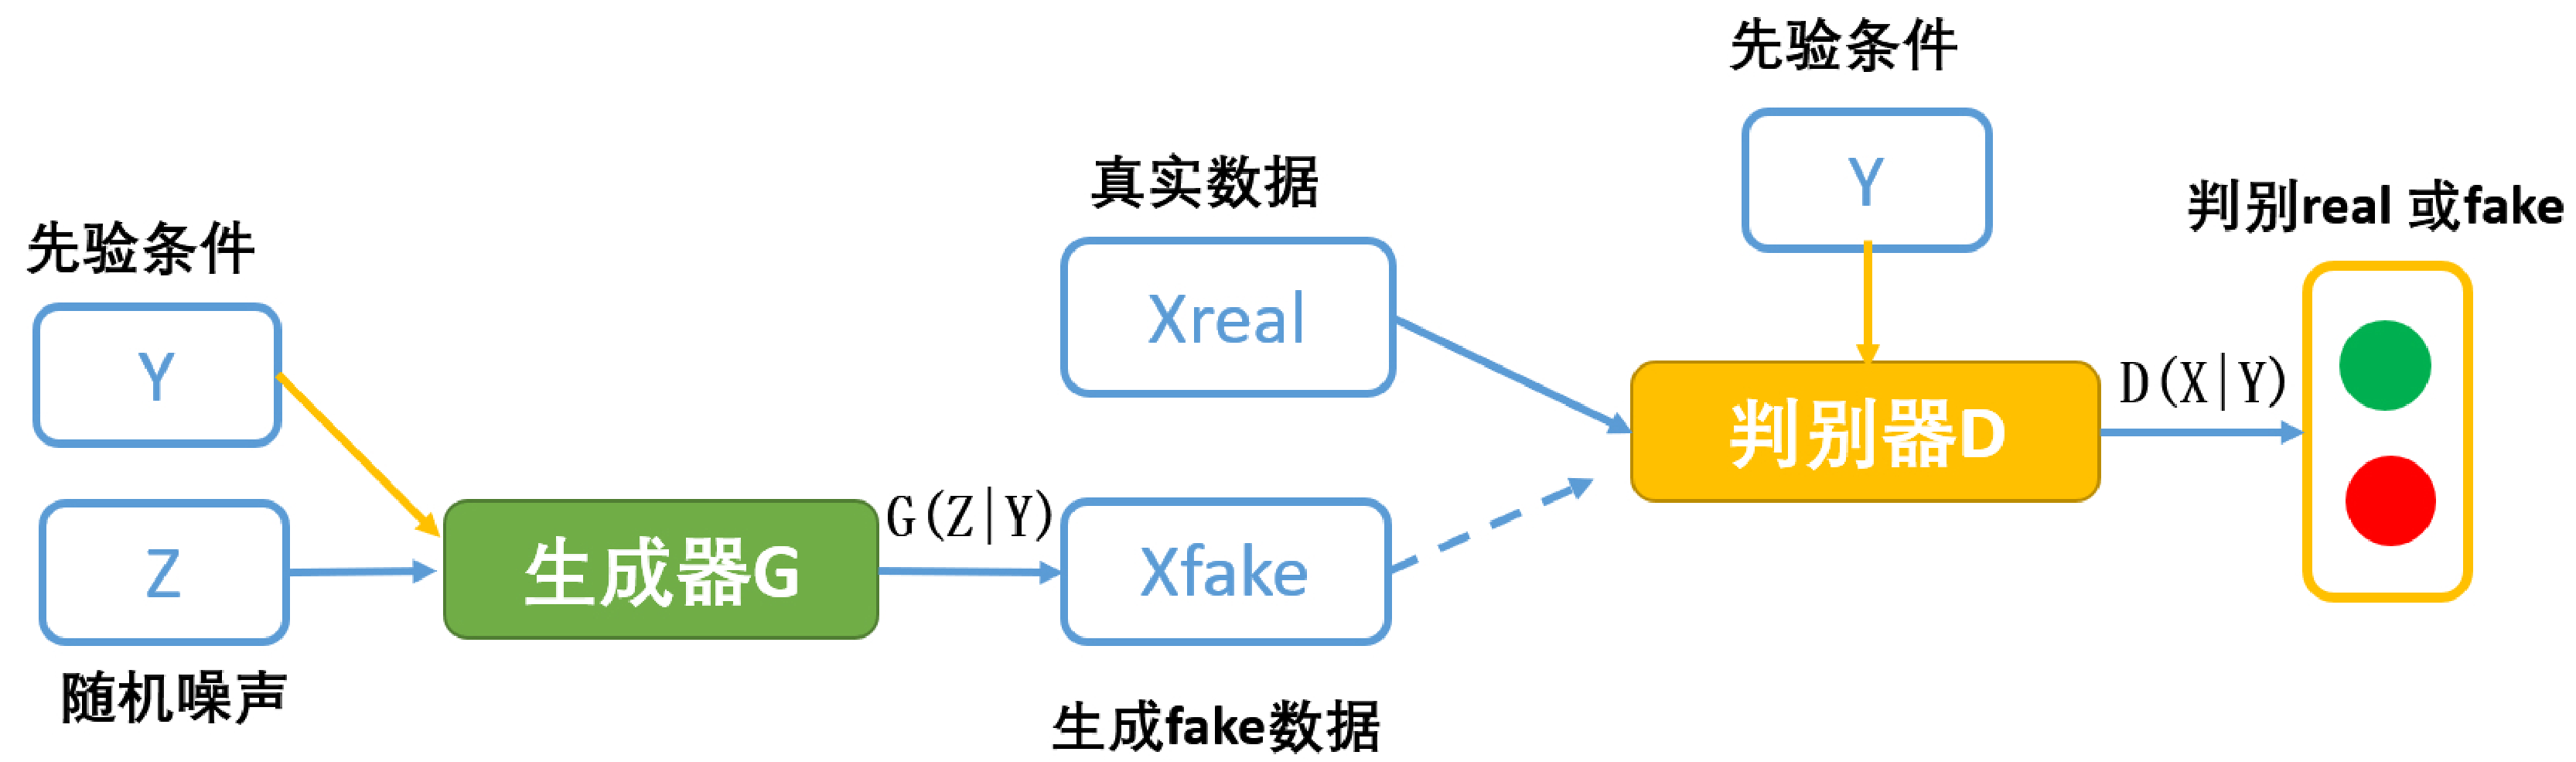
\includegraphics[width=0.8\textwidth]{figures/cgan}
  \caption{CGAN结构示意图}\label{fig:cgan}
\end{figure}

CGAN 模型中,生成器G 中随机噪声$z$与条件先验知识$y$ 被联合组成联合隐层输入特征;判别器D 中$X$ 和$y$ 通过词嵌入共同作为模型输入。 类似式\ref{eq:4-1}, CGAN 模型目标函数为带有条件概率的二人极小极大值博弈函数,即:

\begin{equation}
  \label{eq:4-3}
  \mathop{\min}_{G} \mathop{\max}_{D} V(D,G) = \mathop{\min}_{G} \mathop{\max}_{D} E_{x \sim p_{data}(x)} [\log D(x|y)] + E_{z \sim p_{z}(z)}[ \log (1-D(G(z|y)))]
\end{equation}

图\ref{fig:cgan} 为CGAN 的结构示意图,通过将额外条件信息$y$ 分别输送给判别模型和生成模型组成联合隐层表征,作为输入层的一部分,从而指导数据的生成过程。


\subsection{基于CGAN 的语义分割方法}
\label{sec:first-2}


\section{实验数据介绍}
blabala

\section{实验结果与分析}
balabala

\section{本章小结}
balabala